\documentclass[11pt,a4paper]{article}

\usepackage[a4paper, top=0.75in, bottom=0.75in, left=0.80in, right=0.80in]{geometry}
\usepackage[utf8]{inputenc}
\usepackage{graphicx}
\usepackage{booktabs}
\usepackage{amsmath}
\usepackage{hyperref}
\usepackage{caption}
\usepackage{subcaption}
\usepackage{float}
\usepackage{parskip}
\usepackage{titlesec}
\usepackage{xcolor}
\usepackage{microtype}
\usepackage{enumitem}

\setlist{nosep, leftmargin=1.4em}
\setlength{\parskip}{3pt}
\captionsetup{font=small, skip=4pt}
\captionsetup[subfigure]{justification=centering, font=small}

\hypersetup{colorlinks=true,linkcolor=blue!60!black,urlcolor=blue!60!black}

\titleformat{\section}{\normalsize\bfseries}{}{0em}{\thesection\enspace}
\titlespacing{\section}{0pt}{6pt}{2pt}
\titleformat{\subsection}{\small\bfseries}{}{0em}{\thesubsection\enspace}
\titlespacing{\subsection}{0pt}{4pt}{1pt}

\graphicspath{{./outputs/}}
% Auto-generated by generate_report_text.py - do not edit manually.
% Re-run python main.py to update all values.

% -- KNN
\newcommand{\knnBoWAcc}{53.12\%}
\newcommand{\knnBertAcc}{88.06\%}
\newcommand{\knnJumpPP}{35}

% -- Logistic Regression
\newcommand{\lrBoWAcc}{85.94\%}
\newcommand{\lrTfidfAcc}{88.88\%}
\newcommand{\lrSvdAcc}{86.12\%}
\newcommand{\lrBertAcc}{88.62\%}
\newcommand{\lrBertPcaAcc}{89.06\%}
\newcommand{\lrBertImprove}{88.62\% $\to$ 89.06\%}
\newcommand{\lrTfidfDrop}{88.88\% $\to$ 86.12\%}

% -- Linear SVM
\newcommand{\lsvmTfidfAcc}{88.62\%}
\newcommand{\lsvmSvdAcc}{86.00\%}
\newcommand{\lsvmTfidfDrop}{88.62\% $\to$ 86.00\%}
\newcommand{\lsvmBertAcc}{87.38\%}
\newcommand{\lsvmPcaAcc}{88.94\%}

% -- RBF SVM
\newcommand{\rbfBertPcaAcc}{90.19\%}
\newcommand{\rbfBertAcc}{89.19\%}

% -- Best overall
\newcommand{\bestAcc}{90.19\%}
\newcommand{\bestFscore}{90.09\%}
\newcommand{\bestModel}{RBF SVM}
\newcommand{\bestFeat}{Reduced DistilBERT (PCA)}

% -- Variance retention
\newcommand{\bertPcaVar}{85.89\%}
\newcommand{\tfidfSvdVar}{16.19\%}
\newcommand{\glovePcaVar}{100.00\%}

% -- KMeans
\newcommand{\kmBowNmi}{0.0452}
\newcommand{\kmBowAri}{0.0142}
\newcommand{\kmTfidfNmi}{0.2411}
\newcommand{\kmBertNmi}{0.5589}
\newcommand{\kmBertAri}{0.5727}
\newcommand{\kmGloveNmi}{0.4504}
\newcommand{\kmGloveAri}{0.3840}

% -- GloVe
\newcommand{\gloveBestAcc}{87.75\%}
\newcommand{\gloveRbfAcc}{87.75\%}

% -- Confusion matrix
\newcommand{\cmSportsCorrect}{405}
\newcommand{\cmSportsTotal}{408}
\newcommand{\cmBizToSci}{48}
\newcommand{\cmSciToBiz}{26}

% -- Dataset
\newcommand{\nSamples}{8{,}000}
\newcommand{\nClasses}{4}
\newcommand{\nTrain}{6{,}400}
\newcommand{\nTest}{1{,}600}
\newcommand{\vocabSize}{5{,}000}


\begin{document}

%% ── Title ──────────────────────────────────────────────────────────────────
\begin{center}
  {\large\bfseries Statistical Machine Learning — Course Project}\\[0.3em]
  {\normalsize Text Classification: Sparse Features vs Static and Contextual Embeddings}\\[0.5em]
  {\small Sharma Dhruv M Ram \quad|\quad BA2025044 \quad|\quad IIIT Bangalore \quad|\quad April 2026}
\end{center}
\vspace{2pt}\hrule\vspace{5pt}

%% ── 1. Introduction ─────────────────────────────────────────────────────────
\section{Introduction and Dataset}

This project compares classical ML models across three text representation paradigms:
\textit{sparse features} (BoW, TF-IDF), \textit{static dense embeddings} (GloVe\,—\,bonus),
and \textit{contextual embeddings} (DistilBERT). Only classical models are trained; DistilBERT
and GloVe are used strictly as frozen feature extractors. The three-way axis isolates whether
gains come from density alone or from contextual understanding.

\textbf{Dataset.} AG News via Hugging Face, \nSamples{} samples (seed\,=\,42), \nClasses{} balanced
classes (\textit{World, Sports, Business, Sci/Tech}, $\approx$2{,}000 each).
Split: \nTrain{} train / \nTest{} test (80/20, random\_state\,=\,42).

%% ── 2. EDA ──────────────────────────────────────────────────────────────────
\section{Dataset Description and EDA}

\begin{figure}[H]
  \centering
  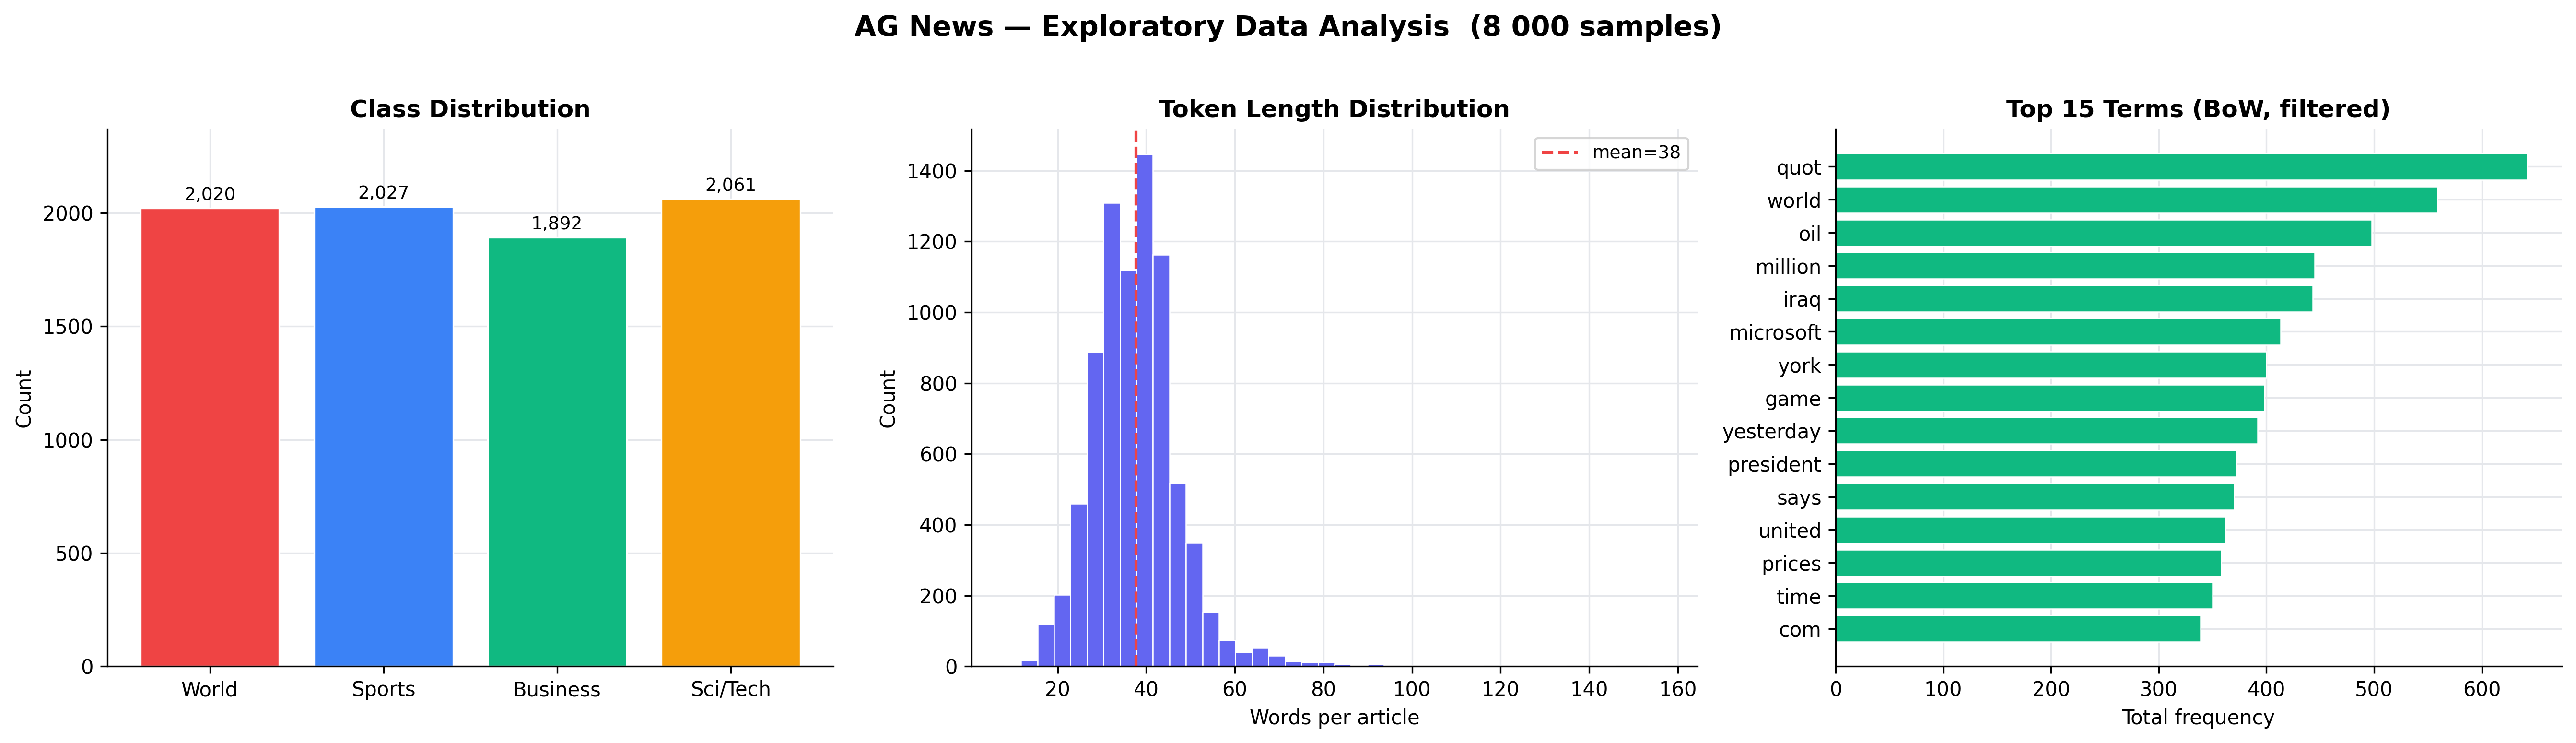
\includegraphics[width=\linewidth]{01_eda_plots.png}
  \vspace{-14pt}
  \caption{EDA: class distribution (balanced), token-length histogram (peak 40–45 words),
           and top-15 BoW terms after stop-word removal.}
  \label{fig:eda}
\end{figure}

The dataset is near-perfectly balanced, eliminating class-imbalance as a confound.
Article lengths follow a roughly Gaussian distribution; very few exceed 100 tokens.
Discriminative vocabulary (extracted from LR coefficients) shows Sports vocabulary is
highly domain-specific, while Business and Sci/Tech share technological terminology
— foreshadowing their classifier confusion.

%% ── 3. Methodology ─────────────────────────────────────────────────────────
\section{Methodology}

\textbf{Part A — Sparse Features.}
\begin{itemize}
  \item \textbf{BoW}: unigram raw-count, top-\vocabSize{} vocab, min\_df\,=\,2, alphabetic tokens $\geq$3 chars.
  \item \textbf{TF-IDF}: unigram+bigram, sublinear\_tf, top-\vocabSize{} vocab, min\_df\,=\,2.
\end{itemize}

\textbf{Part B — GloVe (Bonus).}
100-d glove-wiki-gigaword-100 (6B tokens); documents represented as arithmetic mean of known
word vectors, cached as \texttt{.npy}.

\textbf{Part C — DistilBERT.}
Frozen \texttt{distilbert-base-uncased}; [CLS] token from final hidden state yields a 768-d
vector per article, computed once on GPU (Kaggle) and cached.

\textbf{Part D — Models.}
Logistic Regression (\texttt{max\_iter=1000}), Linear SVM, RBF SVM, KNN ($k$\,=\,5),
KMeans ($K$\,=\,4, unsupervised baseline).

\textbf{Part E — Dimensionality Reduction.}
Truncated SVD on TF-IDF and PCA on DistilBERT/GloVe, all compressed to 100 components.

\begin{figure}[H]
  \centering
  \begin{subfigure}[b]{0.47\linewidth}
    \centering
    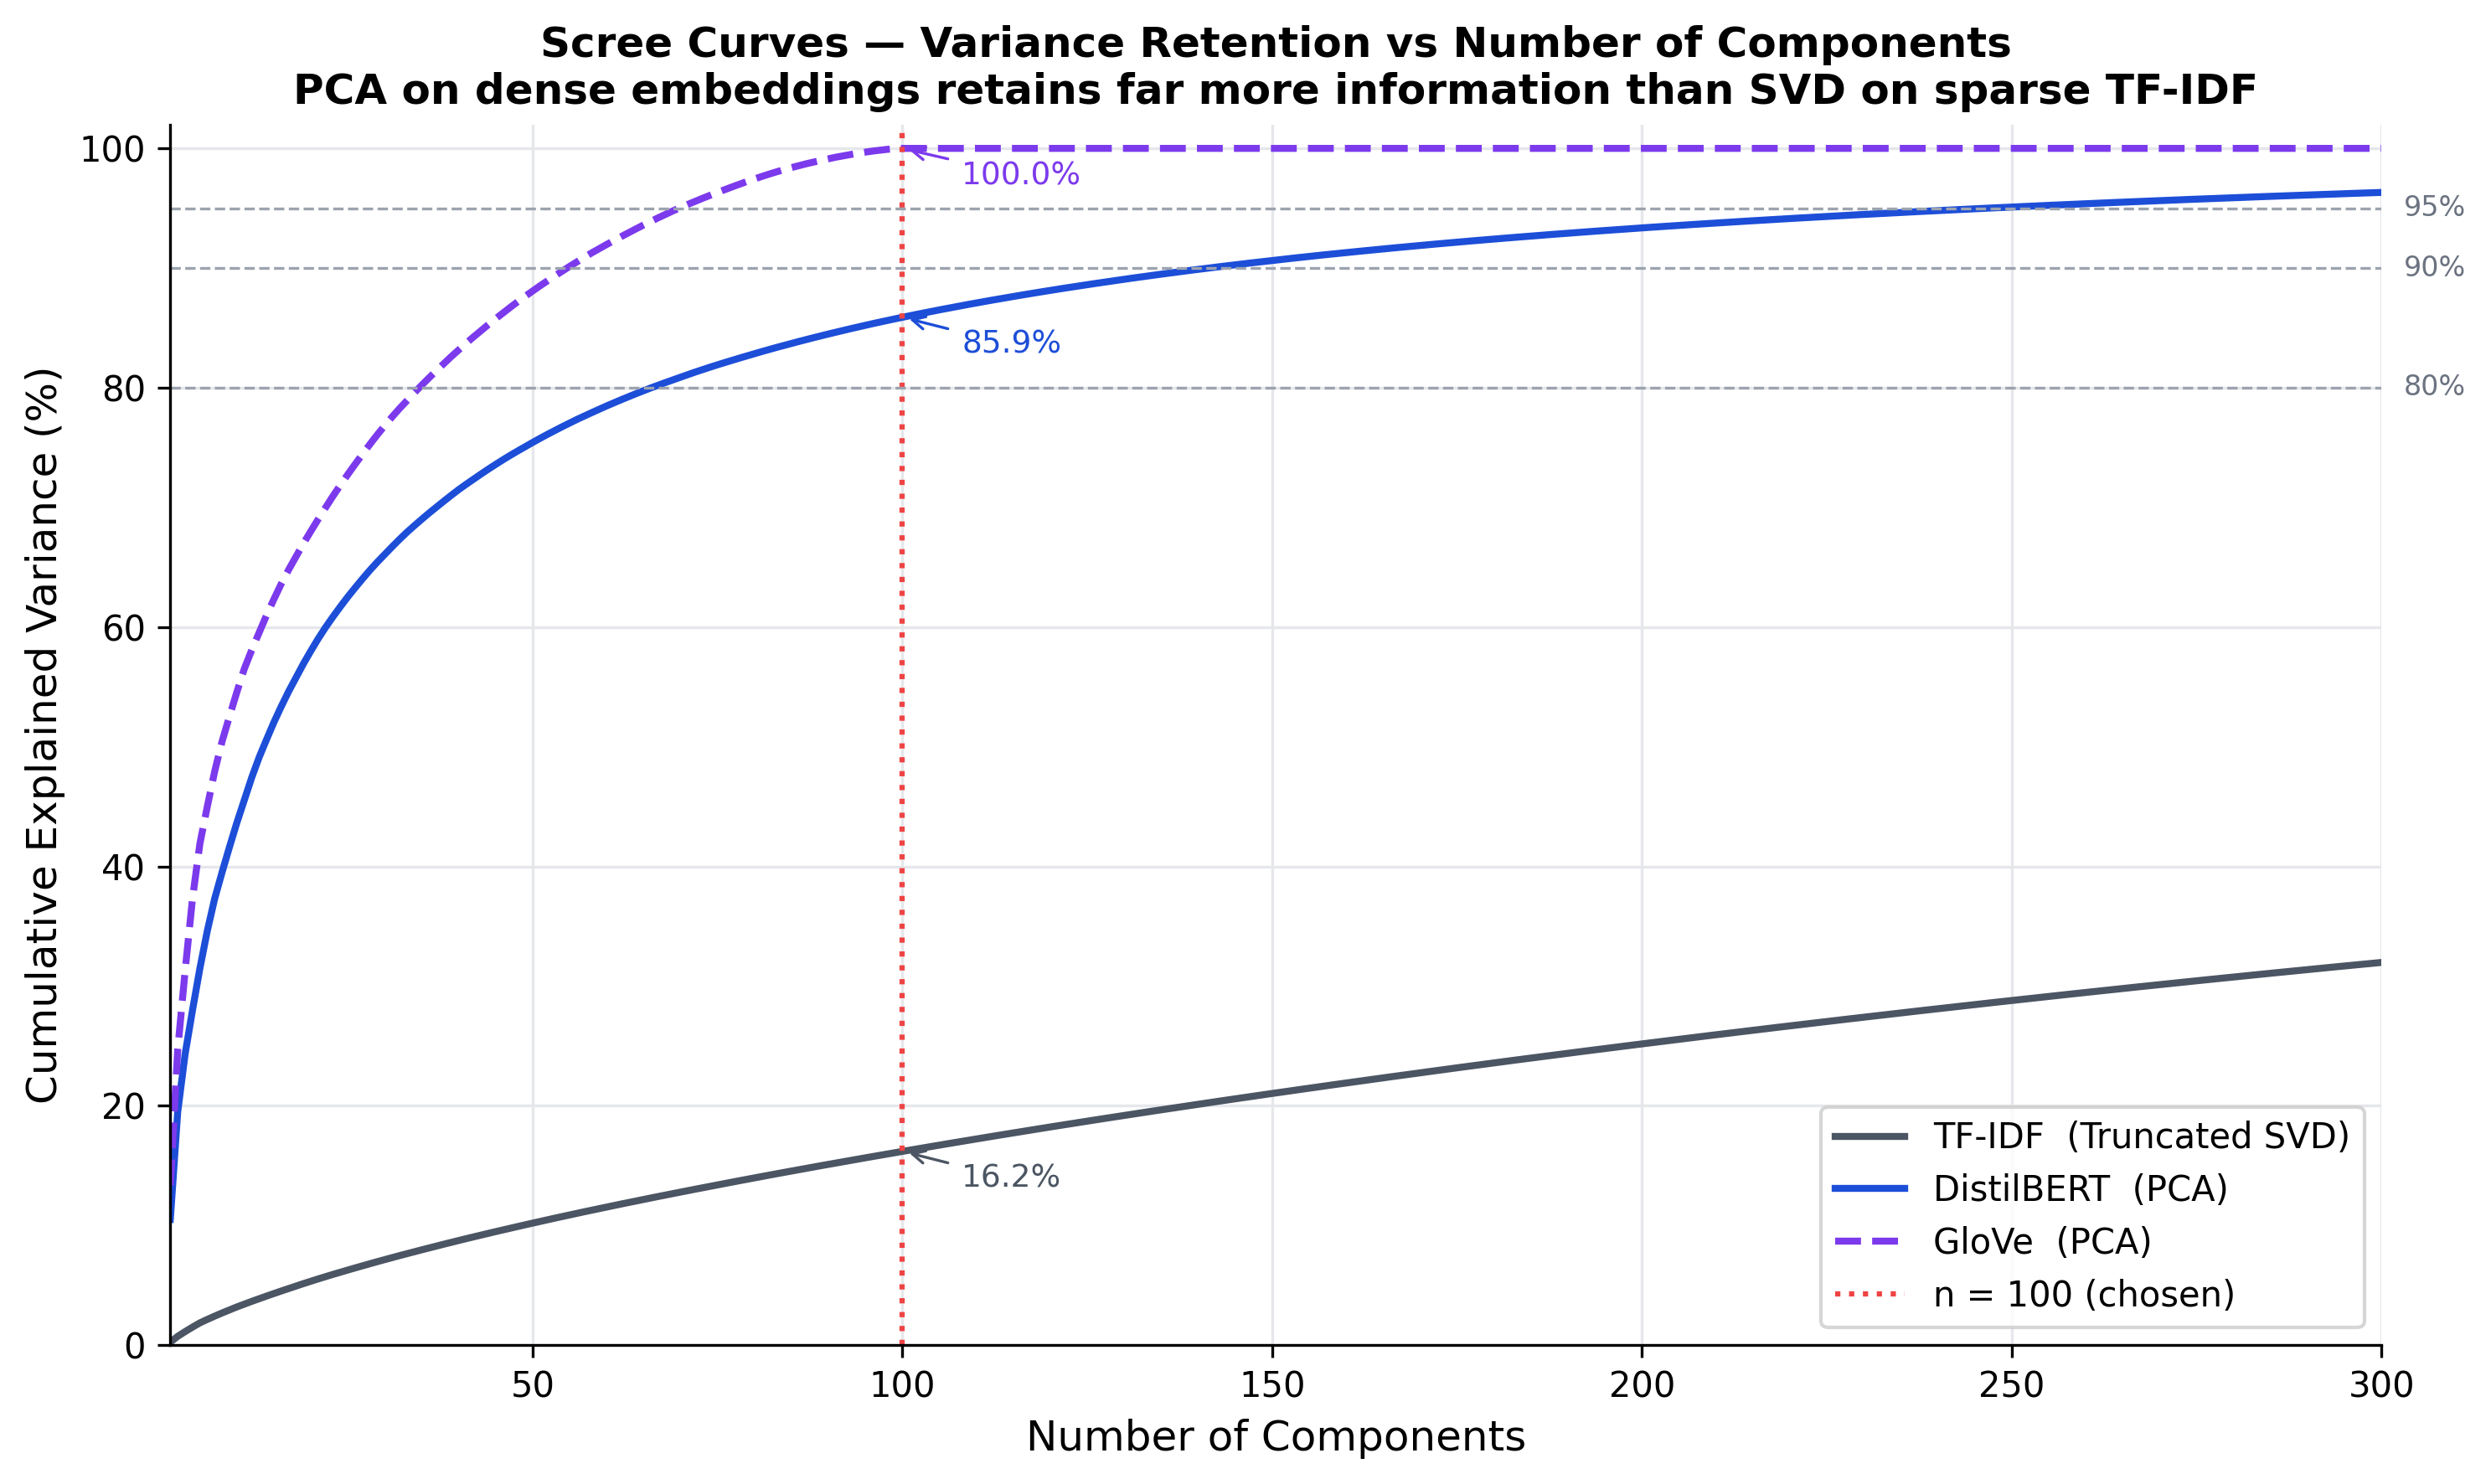
\includegraphics[width=\linewidth]{03_scree_curves.png}
    \caption{Scree curves: PCA retains \bertPcaVar{} of DistilBERT variance at $n{=}100$;
             SVD retains only \tfidfSvdVar{} for TF-IDF.}
    \label{fig:scree}
  \end{subfigure}
  \hfill
  \begin{subfigure}[b]{0.50\linewidth}
    \centering
    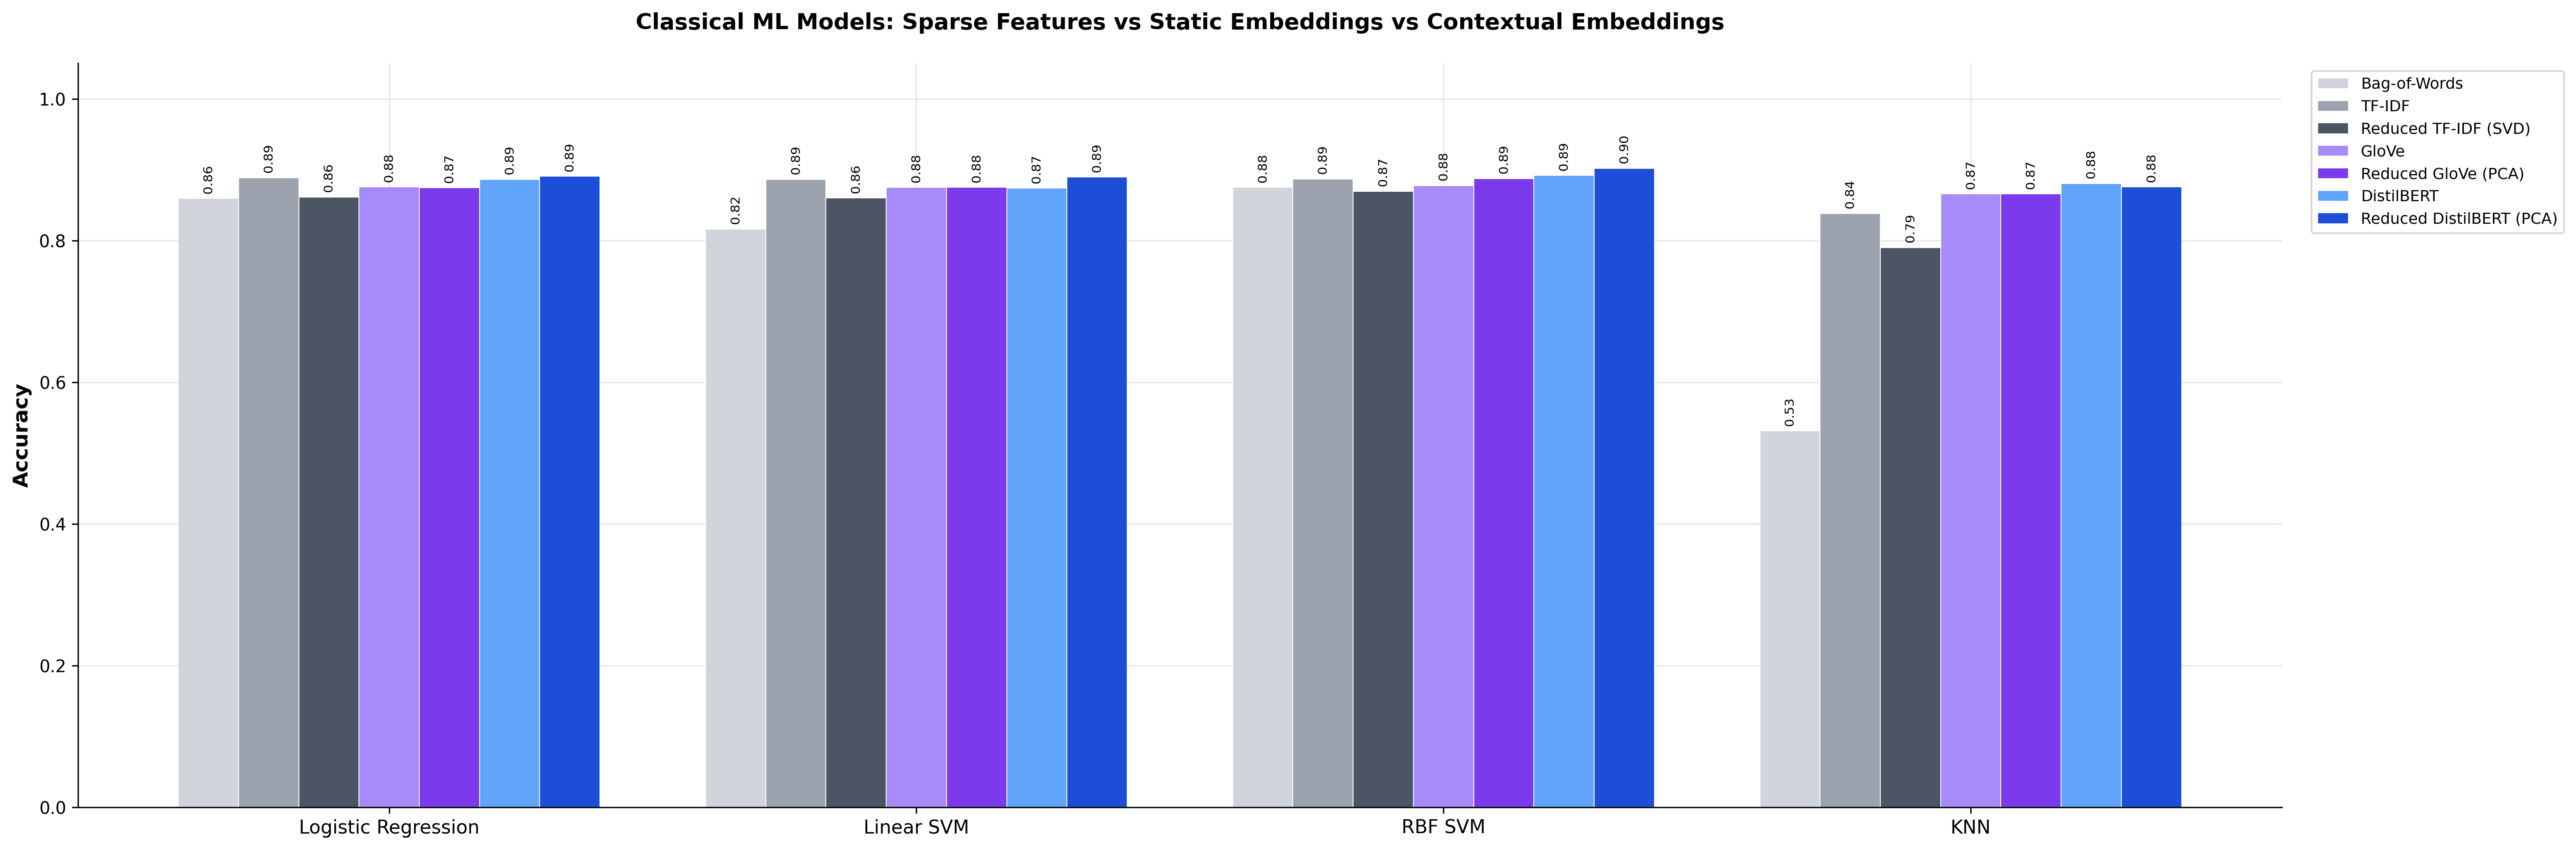
\includegraphics[width=\linewidth]{08_model_comparison.png}
    \caption{Accuracy across all models and feature spaces.
             Sparse $\to$ GloVe $\to$ DistilBERT is consistent.}
    \label{fig:acc}
  \end{subfigure}
  \caption{Dimensionality reduction variance retention (left) and overall accuracy comparison (right).}
\end{figure}

%% ── 4. Experiments ──────────────────────────────────────────────────────────
\section{Experiments}

Each supervised model was trained on an 80/20 stratified split
(\texttt{random\_state=42}) and evaluated on held-out accuracy and macro F1.
KMeans was fit on the full dataset and evaluated via NMI and ARI.
Dimensionality reduction was applied independently per feature space (100 components).

%% ── 5. Results ──────────────────────────────────────────────────────────────
\section{Results}

\subsection{Full Numerical Results}

\begin{table}[H]
\centering
\caption{Accuracy and Macro F1-score for all model--feature combinations. Best per model in \textbf{bold}.}
\label{tab:results}
\renewcommand{\arraystretch}{1.1}
\footnotesize
\begin{tabular}{llcc}
\toprule
\textbf{Model} & \textbf{Feature Set} & \textbf{Accuracy} & \textbf{Macro F1} \\
\midrule
Logistic Regression & Bag-of-Words (unigram)            & 0.8594 & 0.8582 \\
Logistic Regression & TF-IDF (unigram+bigram)            & 0.8888 & 0.8874 \\
Logistic Regression & Reduced TF-IDF (SVD, 100d)         & 0.8612 & 0.8596 \\
Logistic Regression & GloVe mean-pool (100d)             & 0.8756 & 0.8745 \\
Logistic Regression & Reduced GloVe (PCA, 100d)          & 0.8744 & 0.8733 \\
Logistic Regression & DistilBERT (768d)                  & 0.8862 & 0.8854 \\
Logistic Regression & Reduced DistilBERT (PCA, 100d)     & \textbf{0.8906} & 0.8895 \\
\midrule
Linear SVM          & Bag-of-Words (unigram)             & 0.8163 & 0.8145 \\
Linear SVM          & TF-IDF (unigram+bigram)            & 0.8862 & 0.8851 \\
Linear SVM          & Reduced TF-IDF (SVD, 100d)         & 0.8600 & 0.8585 \\
Linear SVM          & GloVe mean-pool (100d)             & 0.8750 & 0.8739 \\
Linear SVM          & Reduced GloVe (PCA, 100d)          & 0.8750 & 0.8739 \\
Linear SVM          & DistilBERT (768d)                  & 0.8738 & 0.8723 \\
Linear SVM          & Reduced DistilBERT (PCA, 100d)     & \textbf{0.8894} & 0.8884 \\
\midrule
RBF SVM             & Bag-of-Words (unigram)             & 0.8750 & 0.8737 \\
RBF SVM             & TF-IDF (unigram+bigram)            & 0.8869 & 0.8856 \\
RBF SVM             & Reduced TF-IDF (SVD, 100d)         & 0.8694 & 0.8682 \\
RBF SVM             & GloVe mean-pool (100d)             & 0.8775 & 0.8766 \\
RBF SVM             & Reduced GloVe (PCA, 100d)          & 0.8875 & 0.8866 \\
RBF SVM             & DistilBERT (768d)                  & 0.8919 & 0.8908 \\
RBF SVM             & Reduced DistilBERT (PCA, 100d)     & \textbf{0.9019} & 0.9009 \\
\midrule
KNN                 & Bag-of-Words (unigram)             & 0.5312 & 0.5309 \\
KNN                 & TF-IDF (unigram+bigram)            & 0.8381 & 0.8361 \\
KNN                 & Reduced TF-IDF (SVD, 100d)         & 0.7900 & 0.7876 \\
KNN                 & GloVe mean-pool (100d)             & 0.8656 & 0.8640 \\
KNN                 & Reduced GloVe (PCA, 100d)          & 0.8656 & 0.8640 \\
KNN                 & DistilBERT (768d)                  & \textbf{0.8806} & 0.8792 \\
KNN                 & Reduced DistilBERT (PCA, 100d)     & 0.8756 & 0.8741 \\
\bottomrule
\end{tabular}
\end{table}

\vspace{-2pt}
\noindent\small KMeans (unsupervised): BoW NMI\,=\,\kmBowNmi, ARI\,=\,\kmBowAri\quad
TF-IDF NMI\,=\,\kmTfidfNmi\quad
DistilBERT NMI\,=\,\kmBertNmi, ARI\,=\,\kmBertAri\quad
GloVe NMI\,=\,\kmGloveNmi, ARI\,=\,\kmGloveAri.

\subsection{Per-Class F1 and Error Analysis}

\begin{figure}[H]
  \centering
  \begin{subfigure}[b]{0.58\linewidth}
    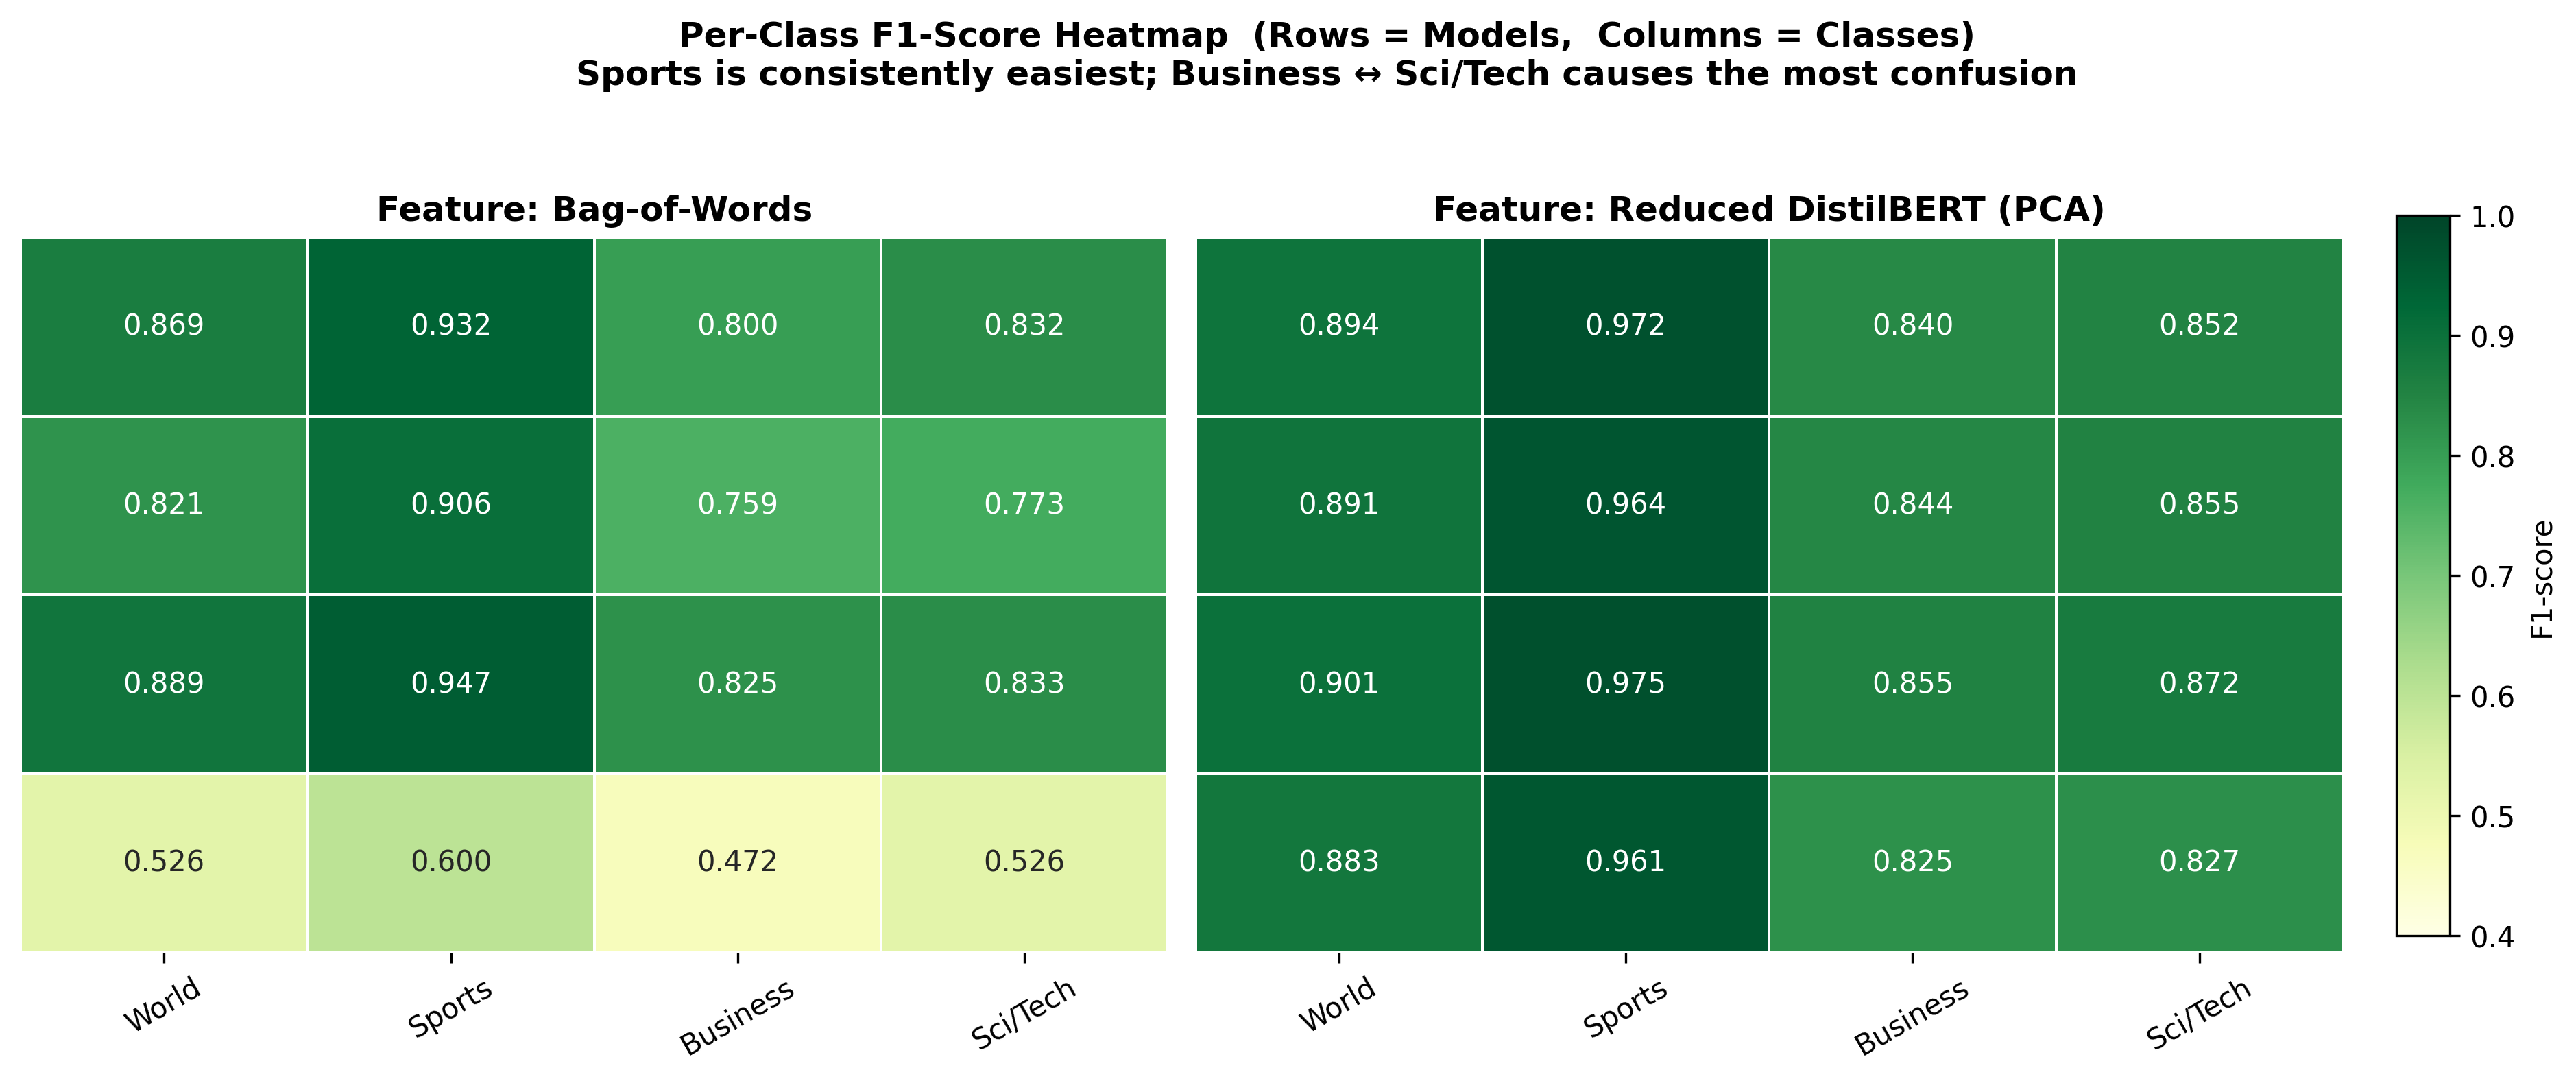
\includegraphics[width=\linewidth]{09_per_class_f1_heatmap.png}
    \caption{Per-class F1: BoW (left) vs Reduced DistilBERT PCA (right).
             Sports easiest; Business/Sci/Tech confusion persists.}
    \label{fig:f1}
  \end{subfigure}
  \hfill
  \begin{subfigure}[b]{0.39\linewidth}
    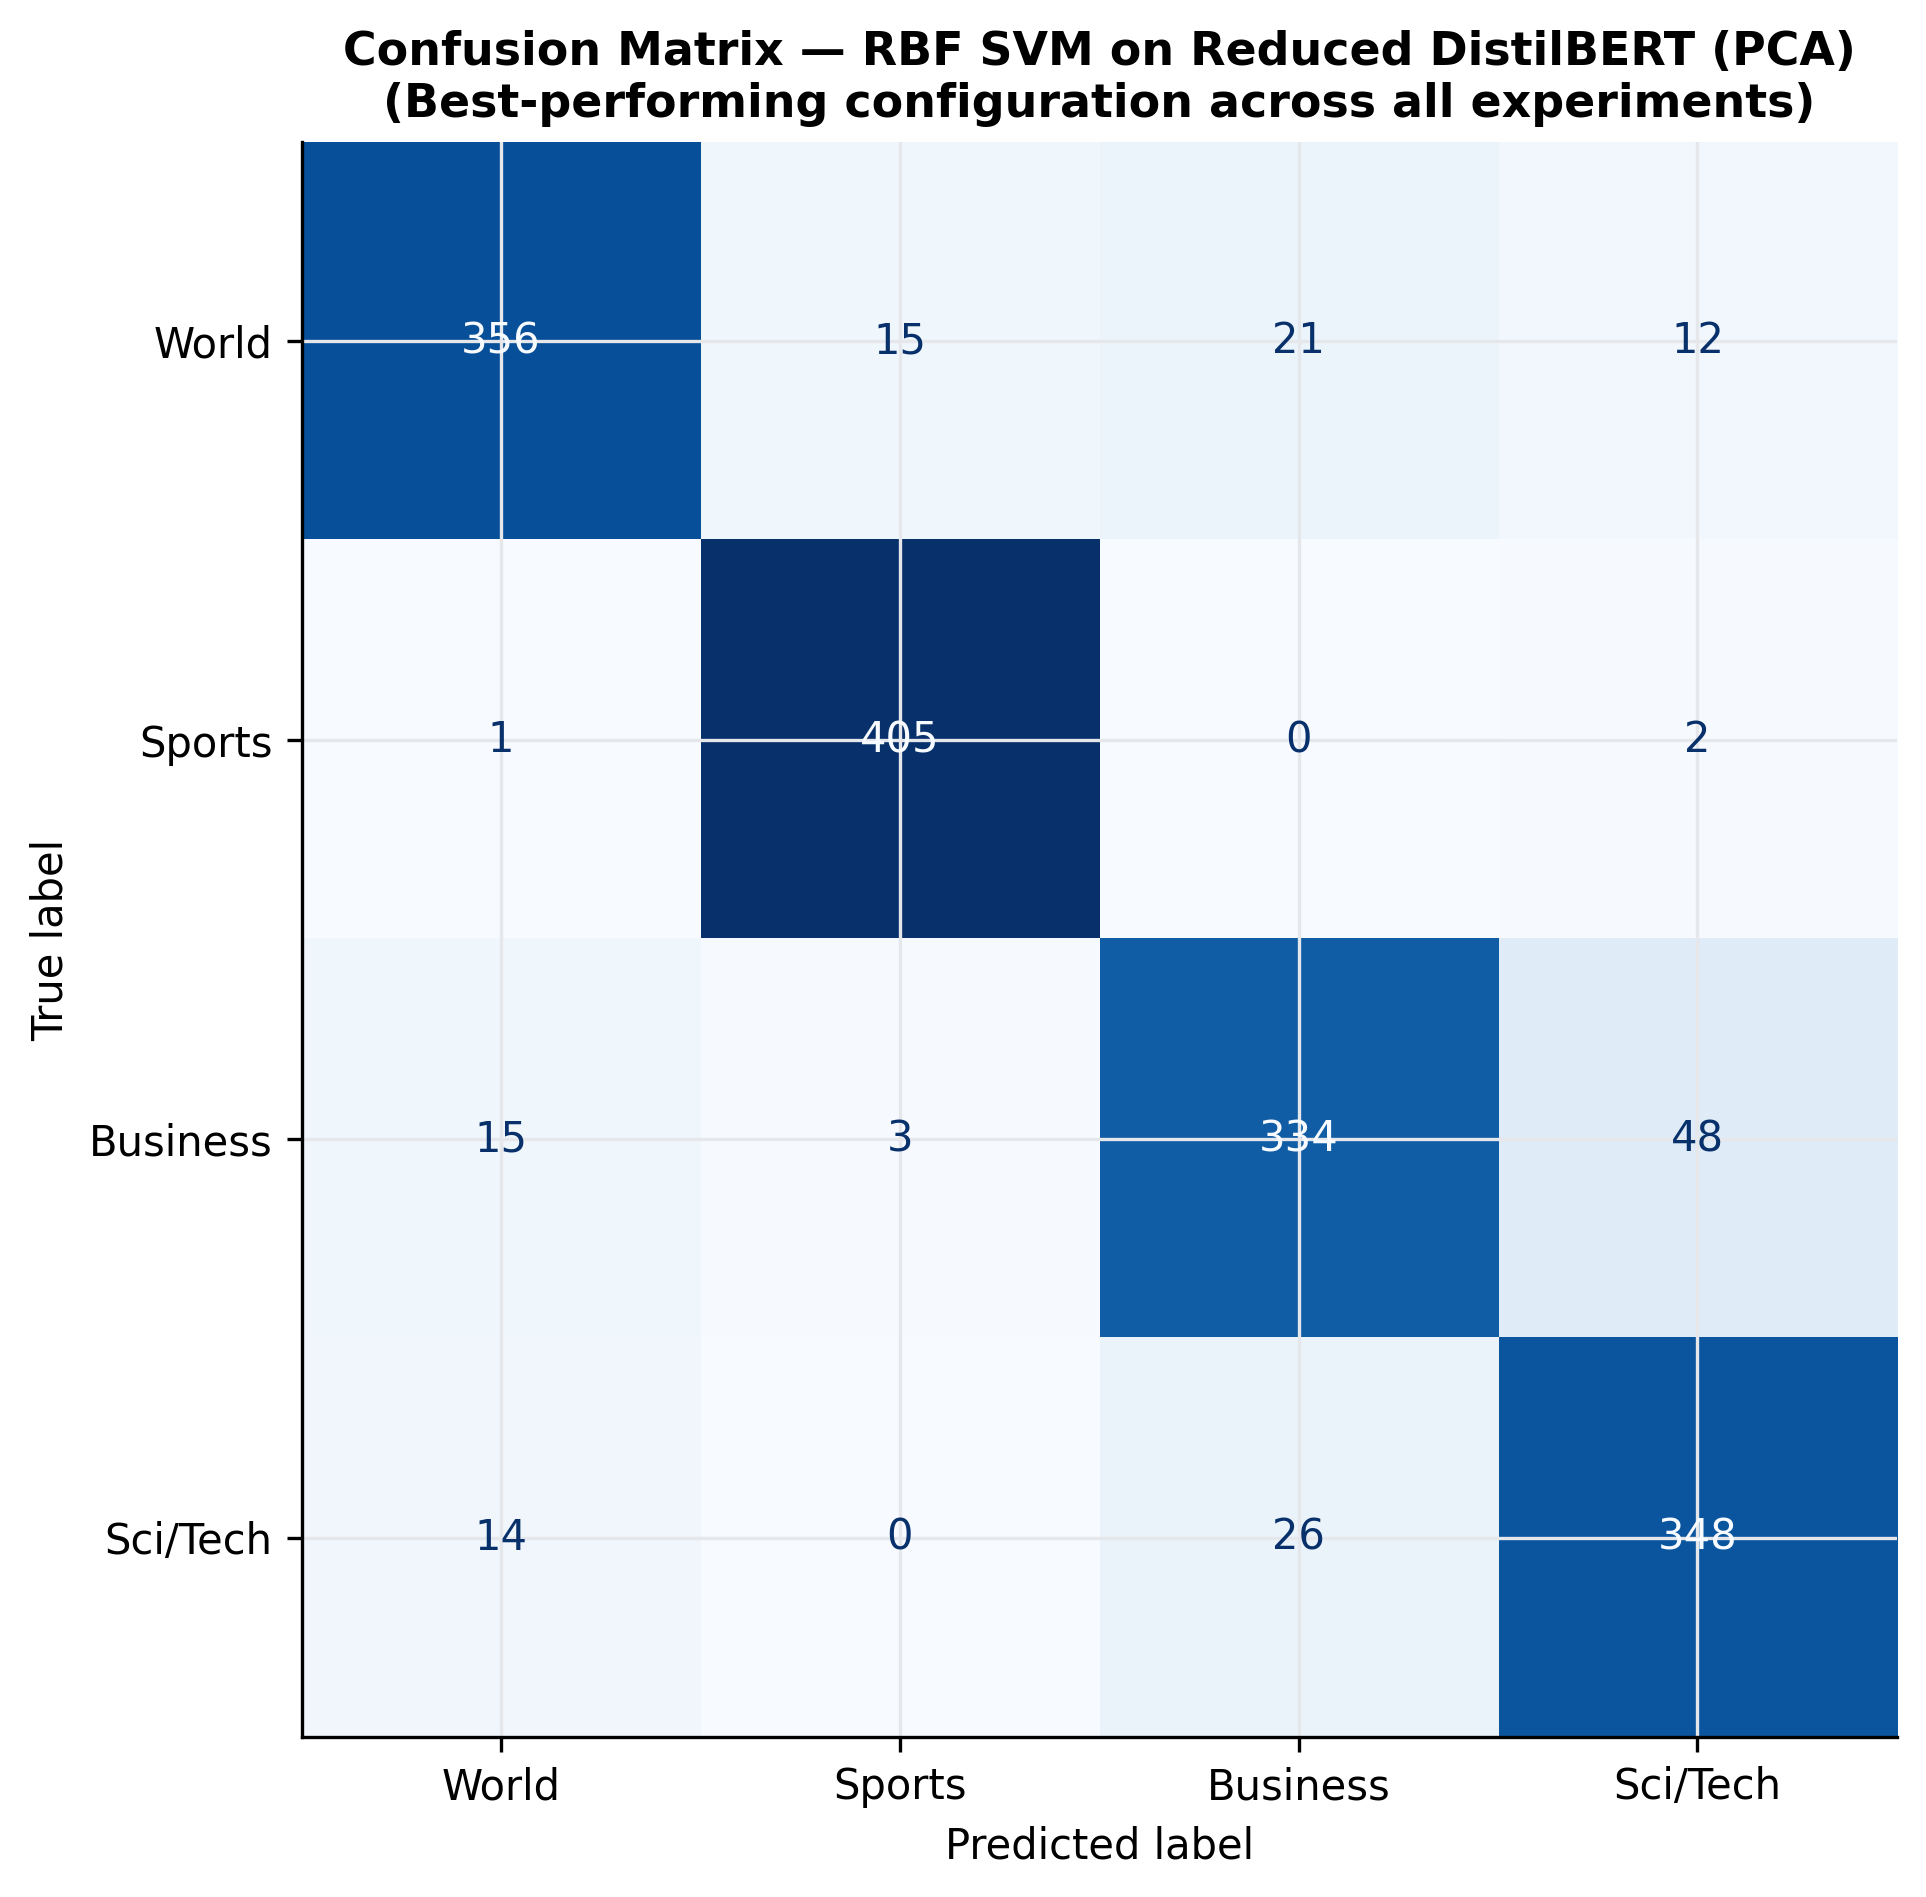
\includegraphics[width=\linewidth]{07_confusion_matrix.png}
    \caption{\bestModel{} on \bestFeat{} (\bestAcc{}).
             Sports \cmSportsCorrect/\cmSportsTotal{}; primary error: \cmBizToSci{}
             Business$\to$Sci/Tech.}
    \label{fig:cm}
  \end{subfigure}
  \caption{Per-class F1 heatmap (left) and best-model confusion matrix (right).}
\end{figure}

%% ── 6. Discussion ───────────────────────────────────────────────────────────
\section{Discussion}

\textbf{Curse of dimensionality.}
KNN on 5{,}000-d sparse BoW scores only \knnBoWAcc{}; on dense 768-d DistilBERT it reaches
\knnBertAcc{} — a \knnJumpPP-point gain from feature change alone.

\textbf{Compression behaviour.}
PCA retains \bertPcaVar{} of DistilBERT variance in 100 components, allowing LR to
\textit{improve} (\lrBertImprove). SVD on TF-IDF retains only \tfidfSvdVar{}, causing a moderate
drop (\lrTfidfDrop). Compression is safe for structured dense embeddings; destructive for
isotropic sparse representations.

\textbf{GloVe as semantic bridge.}
RBF SVM reaches \gloveRbfAcc{} on GloVe vs \rbfBertPcaAcc{} on Reduced DistilBERT.
The gap isolates the contribution of \textit{contextual} disambiguation, not density.
The full hierarchy is: BoW $<$ TF-IDF $<$ GloVe $<$ DistilBERT, mapping directly to
no-semantics $\to$ co-occurrence $\to$ static word semantics $\to$ contextual sentence semantics.

\textbf{Class-level confusion.}
Sports is the easiest class due to highly domain-specific vocabulary. \cmBizToSci{} Business
articles are misclassified as Sci/Tech — modern tech-company news genuinely straddles both
domains. This confusion hierarchy is preserved across all feature spaces.

\textbf{KMeans as unsupervised probe.}
DistilBERT achieves NMI\,=\,\kmBertNmi{} and ARI\,=\,\kmBertAri{} \textit{without any classifier},
vs NMI\,=\,\kmBowNmi{} for BoW — confirming the class separation is a geometric property of
the embedding space, not a classifier artefact.

\textbf{Limitations.}
Single 80/20 split (no cross-validation for main results); default sklearn hyperparameters
throughout; GloVe mean-pooling ignores word order; DistilBERT CLS token only (mean-pooling
often more robust).

%% ── 7. Conclusion ───────────────────────────────────────────────────────────
\section{Conclusion and Learnings}

The best configuration is \textbf{\bestModel{} on \bestFeat{}} at \textbf{\bestAcc{}}
(Macro F1\,=\,\bestFscore{}). Classical ML performance is bounded by input feature quality:
provide a good feature space and even simple models excel. PCA on DistilBERT is
information-preserving (\bertPcaVar{} retention) and actually improves downstream accuracy
by removing noise; SVD on TF-IDF is destructive (\tfidfSvdVar{} retention) because sparse
representations lack low-rank structure. DistilBERT's advantage over GloVe is attributable
to contextual disambiguation, not mere density, as the GloVe baseline eliminates density
as a confound.

\end{document}